\chapter{Experimentación: modelos \\ y entrenamiento}

En este capítulo usaremos todos los conceptos vistos en los capítulos anteriores para justificar las elecciones de los diferentes modelos, hablaremos de las características principales de los mismos y finalmente entraremos en la fase del entrenamiento y los resultados de dichos modelos.

\begin{figure}[h]
	\centering
	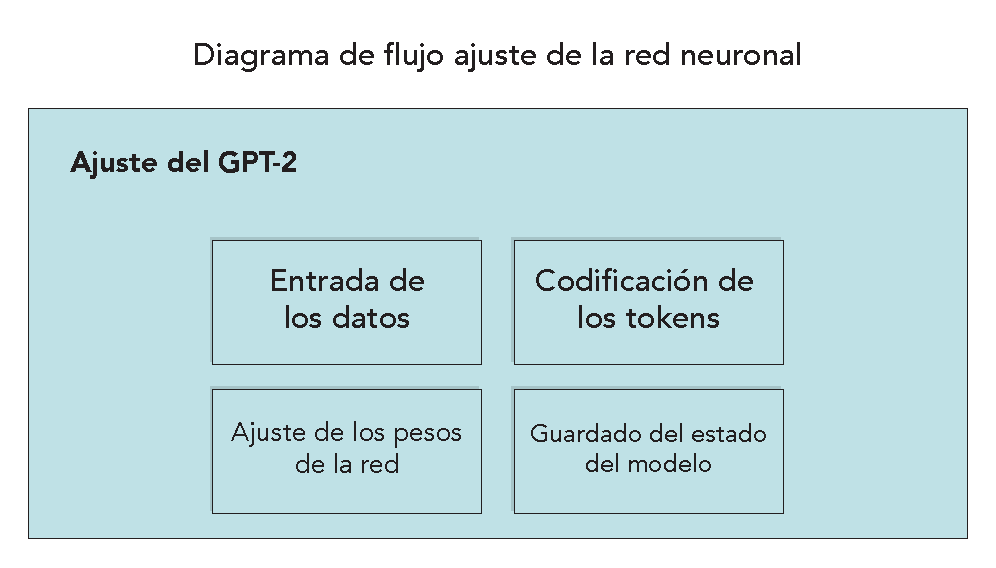
\includegraphics[width=.9\textwidth]{media/gpt-fine-tune.pdf}
	\caption{Diagrama resumen del ajuste de los pesos del GPT2}
	\label{fig:fine-tune-gpt}
\end{figure}

En la figura \ref{fig:fine-tune-gpt} podemos ver un breve resumen de las diferentes tareas de las que se compone el entrenamiento del modelo. Pasaremos a explicar en profundidad cada una de esas subtareas en las siguientes secciones.


\section{Experimentación}
En esta sección describiremos los diferentes pasos que fue necesario acometer para el entrenamiento del modelo del GPT2, el transformer que hemos utilizado para nuestro proyecto.

\subsection{Entrada de los datos}
En primer lugar, debemos ofrecer los datos de entrada al modelo. Estos datos están previamente formateados y unificados, como vimos en la fase de preprocesamiento.

Es importante la adición de las etiquetas \jesitt{<|BOS|>} y \jesitt{<|EOS|>}. Estas etiquetas son las siglas de \textit{begin of sentence} y \textit{end of sentence}. Son marcadores que indican, como es obvio, el inicio y fin de una oración. Estas etiquetas son necesarias para que el modelo entienda cuál es el criterio a partir del cual empieza y acaba una oración.

\subsection{Codificación de los tokens}
Antes de pasar los datos al modelo, debemos codificarlos. Codificar significa obtener un código único en función del token que estemos considerando. La codificación es esencial para estos modelos, ya que ofrece una representación matemática de las palabras. La codificación de los tokens se efectúa mediante un diccionario preentrenado, de forma que la codificación decodificación sean consistentes, dado un modelo determinado.


\subsection{Ajuste de los pesos}
Nuestro modelo ya está construido. Esto es, los diseñadores ya han decidido las distintas capas y el orden de estas según hemos visto en las secciones anteriores. Este modelo se nos ofrece preentrenado de forma bastante simple. Tal y como viene en el paquete, es capaz de generar frases con relativo sentido, es decir, de algún modo \textit{sabe hablar}. El ajuste se efectúa como un proceso de aprendizaje no supervisado, en la que exponemos a la red a un conjunto de comentarios de forma que ésta podrá generar nuevos comentarios de la nada que caigan bajo la función de distribución de los comentarios de entrada. 

En nuestro caso, esta \textit{función de distribución} la define nuestro conjunto de datos de informes médicos. Este proceso efectivamente ajusta los pesos de la red de forma que se familiarice al modelo con el vocabulario y expresiones comunes encontradas en nuestro conjunto de datos.

Como sabemos, este proceso es, computacionalmente, extraordinariamente costoso. Debemos calcular el peso de millones de parámetros (117 millones en nuestro caso particular), debido a la magnitud del modelo. Para ello, hemos de tener disponible un equipo con, como mínimo, una tarjeta gráfica decente que nos permita hacer cálculos matriciales en paralelo, operaciones muy comunes en el entrenamiento de las redes neuronales.

Dichos equipos pueden ser muy caros. Para ello, hicimos uso del servicio de clústeres de la UGR, enviando nuestros datos mediante \jesitt{ssh}, entrenando el modelo, y descargándonoslos de vuelta.

\subsection{Guardado del estado del modelo}
Finalmente, una vez entrenado el modelo, lo más importante es guardar su estado. Esto es muy fácil gracias a los métodos provistos por las librerías de deep learning. Este estado se guarda en un archivo, que, generalmente, consta de un diccionario en el que las claves corresponden a los nodos de las capas en sí, es decir, a sus parámetros entrenables, y cuyo valor es el peso de dicho nodo. 

De esta forma, es fácil cargar un modelo \textit{vacío}, un modelo inicializado con pesos nulos o no relevantes, y sustituir dichos valores por los incluidos en el archivo. Esto nos permite volver al estado en el que dejamos al modelo tras el costoso entrenamiento.

\section{Generación de comentarios}

\begin{figure}[h]
	\centering
	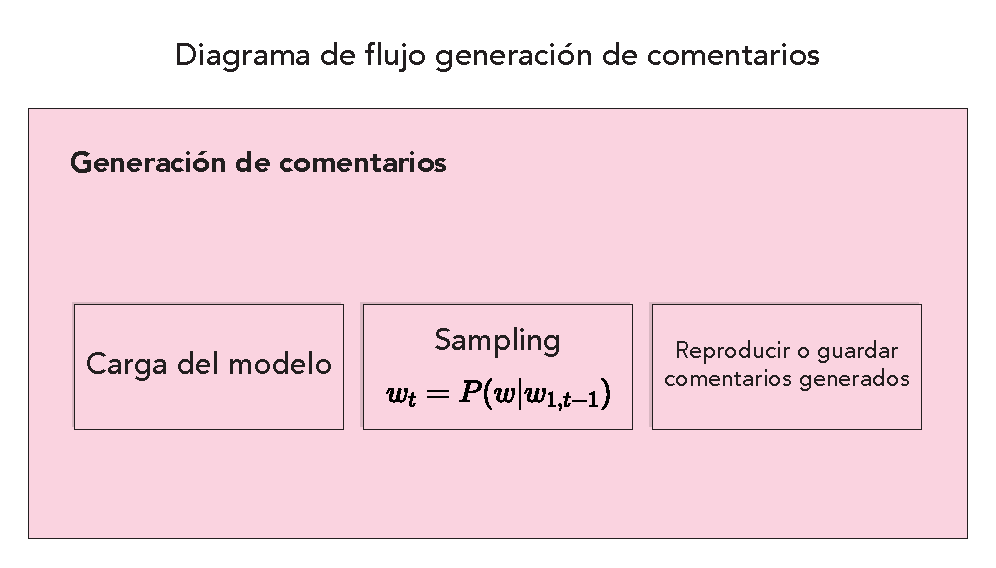
\includegraphics[width=.9\textwidth]{media/comment-gen.pdf}
	\caption{Diagrama resumen de la generación de comentarios}
	\label{fig:comment-gen}
\end{figure}

En esta sección hablaremos de la generación de comentarios, una vez nuestro modelo está entrenado y listo para funcionar. 

\subsection{Carga del modelo}
Como indicamos anteriomente, la carga del modelo es realmente sencilla gracias a las librerías que lo hacen posible. Con nuestro archivo con los pesos localizado, podemos cargar de vuelta los pesos relevantes en los parámetros correspondientes de la red, recuperando el estado original. Este estado es el que nos permitirá generar comentarios de forma automática.

\subsection{Sampling y otros métodos de generación de texto}
Ahora que nuestro modelo está listo, podremos generar comentarios de la nada, casi como por \textit{arte de magia}. Aún así, este proceso no es trivial y merece ser aclarado.

Debemos gran parte de esta sección a la magnífica explicación de Patrick von Platen en su publicación \href{https://huggingface.co/blog/how-to-generate}{How to generate text}. Precisamente es uno de los integrantes de Hugging Face, una empresa de código abierto que se dedica a la creación de los diferentes modelos de los que hemos hablado anteriormente, y que nos ha provisto con una manera fácil y accesible de poder utilizar estas herramientas tan potentes.

Existen varias maneras de generar lo que en la jerga se denomina \textit{texto abierto}, es decir, texto libre sin restricciones. Muchos modelos son capaces de hacerlo, aunque nosotros nos centraremos en los métodos que conciernen al GPT2, que es un modelo autorregresivo.

Los modelos autorregresivos asumen que la siguiente palabra a generar se calcula como una función de probabilidad de todas las palabras anteriores, dada una palabra de contexto inicial.

\subsubsection{Greedy search}
La búsqueda voraz obtiene la palabra con mayor probabilidad de todas las opciones dada una palabra inicial. 





\section{Resultados}